\documentclass{article} % For LaTeX2e
\usepackage{nips15submit_e,times}
\usepackage{hyperref}
\usepackage{graphicx}
\usepackage{url}
%\documentstyle[nips14submit_09,times,art10]{article} % For LaTeX 2.09
\newcommand\BibTeX{B{\sc ib}\TeX}

\title{LSTM for Sentiment Analysis on Twitter}

\author{
Trapit Bansal
\And
Kate Silverstein
\And
Jun Wang
}

%% \author{
%% David S.~Hippocampus\thanks{ Use footnote for providing further information
%% about author (webpage, alternative address)---\emph{not} for acknowledging
%% funding agencies.} \\
%% Department of Computer Science\\
%% Cranberry-Lemon University\\
%% Pittsburgh, PA 15213 \\
%% \texttt{hippo@cs.cranberry-lemon.edu} \\
%% \And
%% Coauthor \\
%% Affiliation \\
%% Address \\
%% \texttt{email} \\
%% \AND
%% Coauthor \\
%% Affiliation \\
%% Address \\
%% \texttt{email} \\
%% \And
%% Coauthor \\
%% Affiliation \\
%% Address \\
%% \texttt{email} \\
%% \And
%% Coauthor \\
%% Affiliation \\
%% Address \\
%% \texttt{email} \\
%% (if needed)\\
%% }


% The \author macro works with any number of authors. There are two commands
% used to separate the names and addresses of multiple authors: \And and \AND.
%
% Using \And between authors leaves it to \LaTeX{} to determine where to break
% the lines. Using \AND forces a linebreak at that point. So, if \LaTeX{}
% puts 3 of 4 authors names on the first line, and the last on the second
% line, try using \AND instead of \And before the third author name.

\newcommand{\fix}{\marginpar{FIX}}
\newcommand{\new}{\marginpar{NEW}}

\nipsfinalcopy % Uncomment for camera-ready version

\begin{document}


\maketitle

\begin{abstract}
abstract goes here
\end{abstract}

\section{Introduction}

We use LSTM \cite{hochreiter1997long} to do stuff

\section{Related Work}

Dynamic convolutional neural net for sentences \cite{kalchbrenner2014convolutional}


sentiment specific word embeddings \cite{tang2014learning}


character-lvl CNN for text classification \cite{zhang2015character}

\section{Model}

\section{Experiments}

\subsection{Datasets}

\subsection{Results}

\begin{table}[h!]
\centering
\caption{Accuracy across LSTMs}
\label{char-models}
\begin{tabular}{|l|ll|}
\hline
              & 1.6M           & semeval \\
\hline
ascii/rnd/50  & \textbf{83.84} & 82.08   \\
ascii/rnd/200 & 82.45          & 83.53   \\
ascii/eye/50  & 77.44          &         \\
utf8          & 81.34          & 82.34   \\
word/rnd      & 81.85          & 78.07   \\
word/sswe     & 83.24          & 79.27   \\
\hline
\end{tabular}
\end{table}




\begin{figure}[h]
\begin{center}
%\framebox[4.0in]{$\;$}
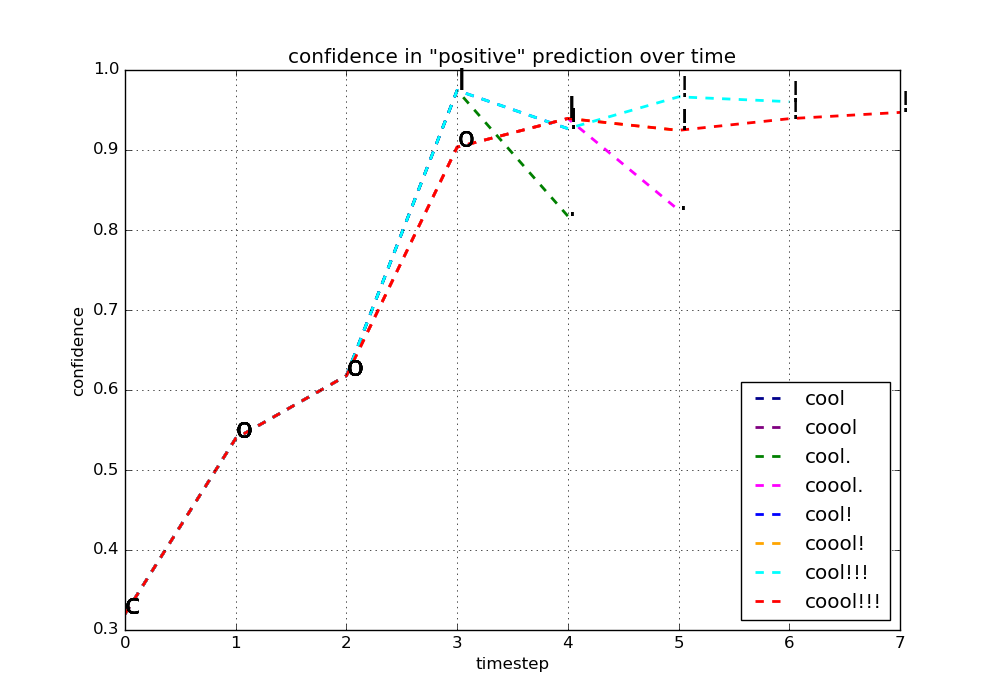
\includegraphics[width=0.95\textwidth]{figs/cool}
%\fbox{\rule[-.5cm]{0cm}{4cm} \rule[-.5cm]{4cm}{0cm}}
\end{center}
\caption{Sample figure caption.}
\end{figure}

\begin{figure}[h]
\begin{center}
%\framebox[4.0in]{$\;$}
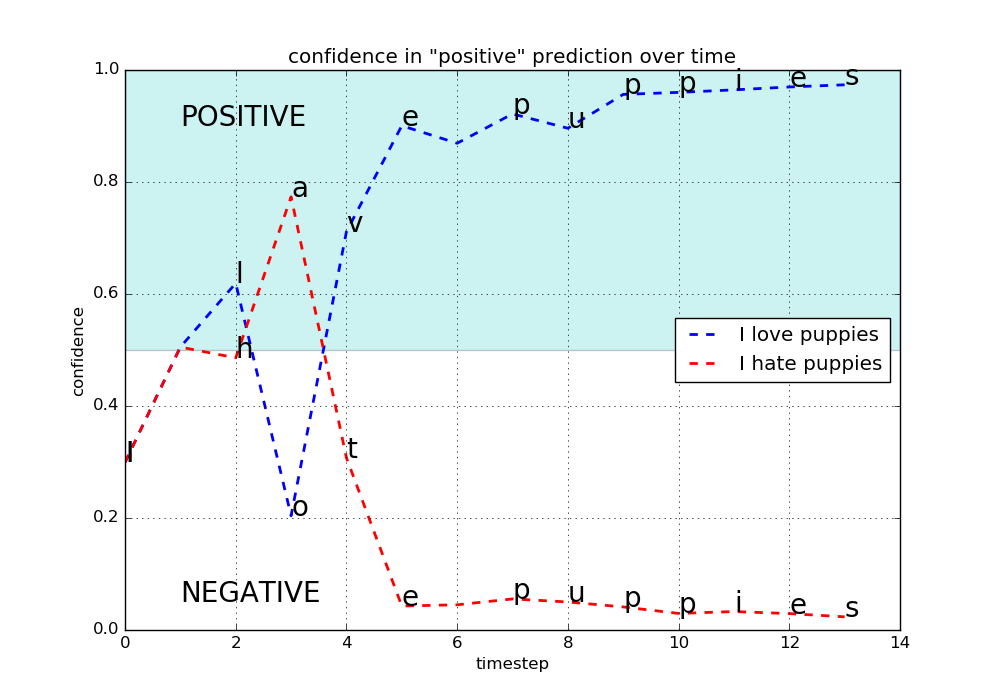
\includegraphics[width=0.95\textwidth]{figs/puppies}
%\fbox{\rule[-.5cm]{0cm}{4cm} \rule[-.5cm]{4cm}{0cm}}
\end{center}
\caption{Sample figure caption.}
\end{figure}

\begin{figure}[h]
\begin{center}
%\framebox[4.0in]{$\;$}
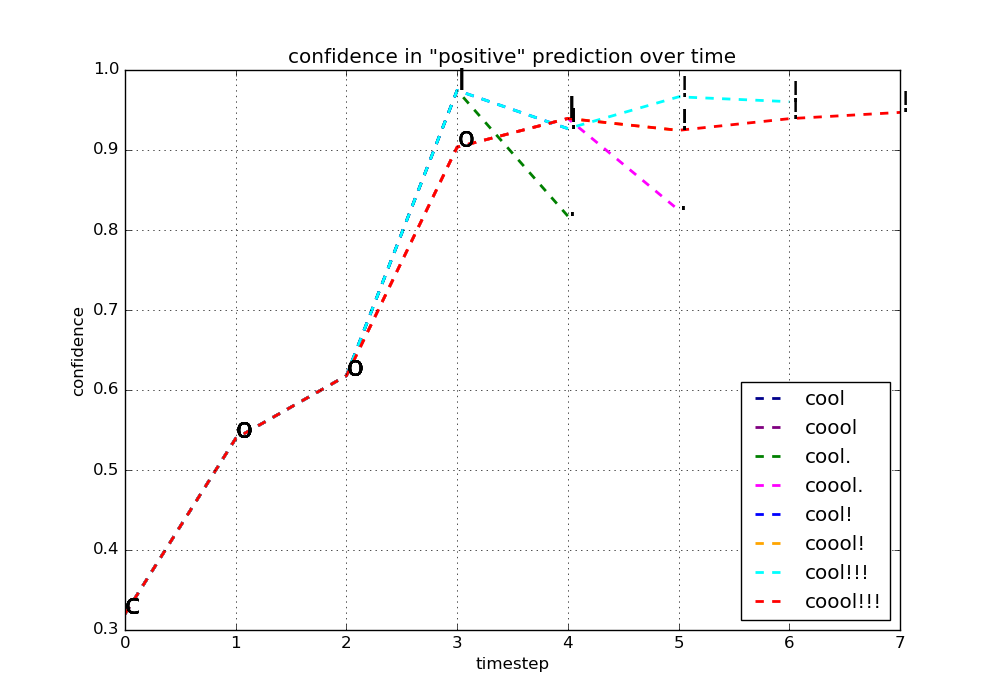
\includegraphics[width=0.95\textwidth]{figs/cool}
%\fbox{\rule[-.5cm]{0cm}{4cm} \rule[-.5cm]{4cm}{0cm}}
\end{center}
\caption{Sample figure caption.}
\end{figure}

\begin{figure}[h]
\begin{center}
%\framebox[4.0in]{$\;$}
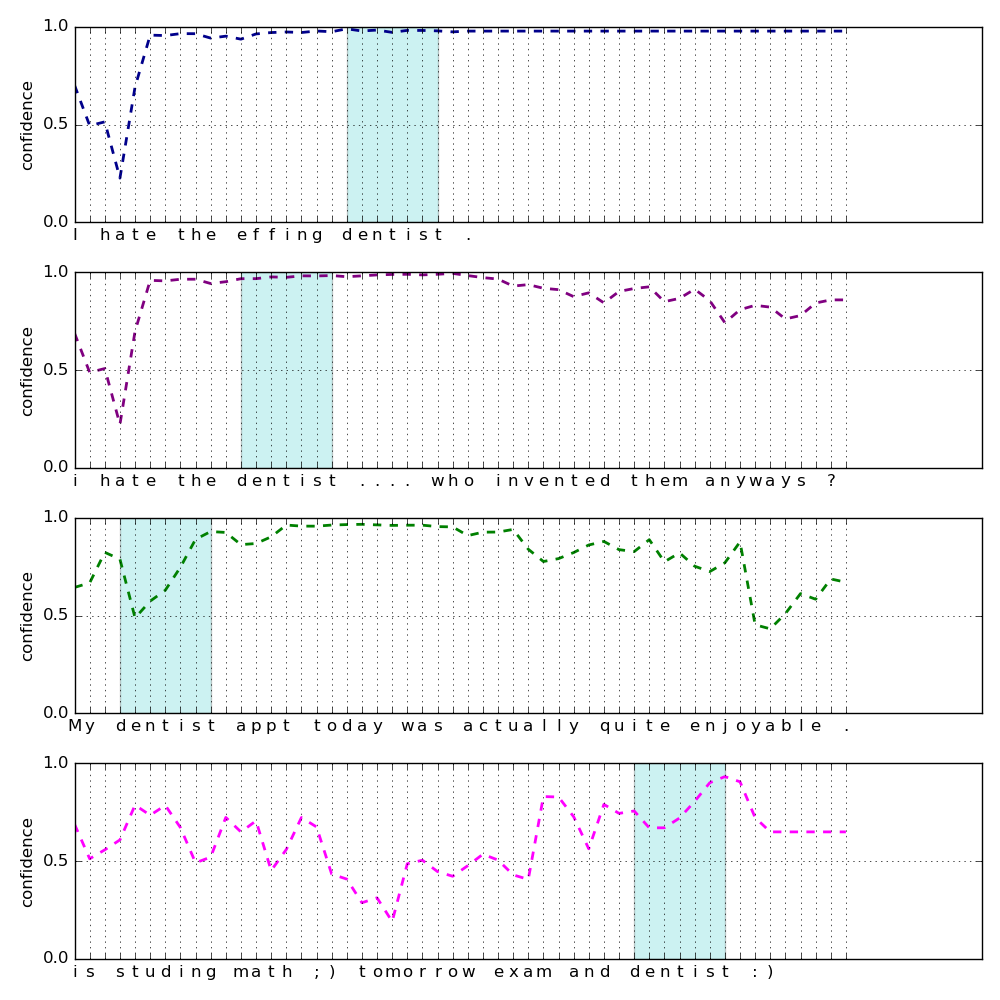
\includegraphics[width=0.95\textwidth]{figs/dentist}
%\fbox{\rule[-.5cm]{0cm}{4cm} \rule[-.5cm]{4cm}{0cm}}
\end{center}
\caption{Confidence in ``negative'' prediction over time}
\end{figure}

\section{Conclusion}


\subsubsection*{Acknowledgments}



\subsubsection*{References}

\bibliography{paper}
\bibliographystyle{plain}
%% References follow the acknowledgments. Use unnumbered third level heading for
%% the references. Any choice of citation style is acceptable as long as you are
%% consistent. It is permissible to reduce the font size to `small' (9-point) 
%% when listing the references. {\bf Remember that this year you can use
%% a ninth page as long as it contains \emph{only} cited references.}

%% \small{
%% [1] Alexander, J.A. \& Mozer, M.C. (1995) Template-based algorithms
%% for connectionist rule extraction. In G. Tesauro, D. S. Touretzky
%% and T.K. Leen (eds.), {\it Advances in Neural Information Processing
%% Systems 7}, pp. 609-616. Cambridge, MA: MIT Press.

%% [2] Bower, J.M. \& Beeman, D. (1995) {\it The Book of GENESIS: Exploring
%% Realistic Neural Models with the GEneral NEural SImulation System.}
%% New York: TELOS/Springer-Verlag.

%% [3] Hasselmo, M.E., Schnell, E. \& Barkai, E. (1995) Dynamics of learning
%% and recall at excitatory recurrent synapses and cholinergic modulation
%% in rat hippocampal region CA3. {\it Journal of Neuroscience}
%% {\bf 15}(7):5249-5262.
%% }

\end{document}
